\section{Results}
\label{results}

\textit{Analysis: of results and the effectiveness of their selection and presentation. Are the results well understood and discussed?}

In this section I am presenting the main results of the current project. I have run code both for generating artificial data set as described in previous sections, as well as on the real one - "file name". 

\subsection{Generated/"Fake" data set}
\subsubsection{OLS, Ridge and Lasso regressions on Franke Function}
For artificial data set, I have used polynomial up to 8th degree with the generated grids of $10\times10$, $21\times21$, $50\times50$ and $100\times100$ points and hyper parameter, $\lambda$, ranging from $0.0001$ to $0.1$. Please note, that such value for the polynomial is not the limited one - the only limitation is the amount of memory on your machine. The results of the runs, for \textit{MSE}s and $R^2$  for two "extreme" cases - $10\times10$ and $100\times100$ are summarized in the tables \ref{table:all-mse1}-\ref{table:all-mse2}. \textbf{Note}: I didn't save these values inside "txt" files, instead they appear directly as a print statements in the console.

\begin{table}[h!]
\begin{tabular}{ |p{2cm}|p{3cm}|p{3cm}|p{3cm}|p{3cm}|  }
 \hline
 \multicolumn{5}{|c|}{Regression Type} \\
 \hline
 Polynomial \newline Degree & Linear \newline MSE, $R^2$ & Ridge \newline MSE, $R^2$ & Lasso \newline MSE, $R^2$  & Type\\
 \hline
 1 & 0.0336, 0.637 \newline 0.0336, 0.637 & 0.0336, 0.637 \newline 0.0336, 0.637 &   0.0336, 0.637 & Scikit Learn \newline Manual\\
 \hline
 2 & 0.0271, 0.707 \newline 0.0271, 0.707  & 0.0271, 0.707 \newline 0.0271, 0.707   & 0.0271, 0.707 & Scikit Learn \newline Manual\\
 \hline
 3 & 0.018, 0.805 \newline 0.018, 0.805 & 0.018, 0.805 \newline 0.018, 0.805 &  0.0186, 0.799 & Scikit Learn \newline Manual\\
 \hline
 4 & 0.0142, 0.846 \newline 0.0142, 0.846 & 0.0142, 0.846 \newline 0.0142, 0.846 &  0.0188, 0.7975 & Scikit Learn \newline Manual\\
 \hline
 5 & 0.0122, 0.868 \newline 0.0122, 0.868 & 0.0122, 0.868 \newline 0.0122, 0.868 & 0.019, 0.7952 & Scikit Learn \newline Manual\\
 \hline
 6 & 0.0111, 0.8800 \newline 0.0111, 0.8800 & 0.01159, 0.8752 \newline 0.01159, 0.8752 & 0.01817, 0.8044 & Scikit Learn \newline Manual\\
 \hline
 7 & 0.01050, 0.8870 \newline 0.01050, 0.8870 & 0.01127, 0.8786 \newline 0.01127, 0.8786 & 0.01740, 0.8126 & Scikit Learn \newline Manual\\
 \hline
 8 & 0.01022, 0.8899 \newline 0.01022, 0.8899 & 0.01118, 0.87967 \newline 0.01118, 0.87967 & 0.01678, 0.81944 & Scikit Learn \newline Manual\\
 \hline
\end{tabular}
\caption{Comparison of results for the fitting of several different regression models to the generated data set. Grid is $10\times10$ points and $\lambda = 0.0001$.}
\label{table:all-mse1}
\end{table}

\begin{table}[h!]
\begin{tabular}{ |p{2cm}|p{3cm}|p{3cm}|p{3cm}|p{3cm}|  }
 \hline
 \multicolumn{5}{|c|}{Regression Type} \\
 \hline
 Polynomial \newline Degree & Linear \newline MSE, $R^2$ & Ridge \newline MSE, $R^2$ & Lasso \newline MSE, $R^2$  & Type\\
 \hline
 1 & 0.0336, 0.637 \newline 0.0336, 0.637 & 0.0336, 0.637 \newline 0.0336, 0.637 &   0.0336, 0.637 & Scikit Learn \newline Manual\\
 \hline
 2 & 0.0271, 0.707 \newline 0.0271, 0.707  & 0.0271, 0.707 \newline 0.0271, 0.707   & 0.0271, 0.707 & Scikit Learn \newline Manual\\
 \hline
 3 & 0.018, 0.805 \newline 0.018, 0.805 & 0.018, 0.805 \newline 0.018, 0.805 &  0.0186, 0.799 & Scikit Learn \newline Manual\\
 \hline
 4 & 0.0142, 0.846 \newline 0.0142, 0.846 & 0.0142, 0.846 \newline 0.0142, 0.846 &  0.0188, 0.7975 & Scikit Learn \newline Manual\\
 \hline
 5 & 0.0122, 0.868 \newline 0.0122, 0.868 & 0.0122, 0.868 \newline 0.0122, 0.868 & 0.019, 0.7952 & Scikit Learn \newline Manual\\
 \hline
 6 & 0.0111, 0.8800 \newline 0.0111, 0.8800 & 0.01159, 0.8752 \newline 0.01159, 0.8752 & 0.01817, 0.8044 & Scikit Learn \newline Manual\\
 \hline
 7 & 0.01050, 0.8870 \newline 0.01050, 0.8870 & 0.01127, 0.8786 \newline 0.01127, 0.8786 & 0.01740, 0.8126 & Scikit Learn \newline Manual\\
 \hline
 8 & 0.01022, 0.8899 \newline 0.01022, 0.8899 & 0.01118, 0.87967 \newline 0.01118, 0.87967 & 0.01678, 0.81944 & Scikit Learn \newline Manual\\
 \hline
\end{tabular}
\caption{Comparison of results for the fitting of several different regression models to the generated data set. Grid is $100\times100$ points and $\lambda = 0.0001$.}
\label{table:all-mse2}
\end{table}

 The first set of values obtained through manual algorithm implementation, while the second row is the comparison to the Scikit Learn. As I've already mentioned before, I have not implemented manual algorithm for Lasso regression, but instead was using only scikit learn functionalities. As we can see, they are almost identical, with the Lasso algorithm being slightly behind. The value $\lambda=0.0001$ is empirical.
 
 Such high values of $R^2$ squared (and low MSE values) are generally a good thing. However, the danger here is that it can be also the sign of the model overfitting. Indeed, in figures \rf{}-\rf{}, you can see the corresponding surfaces of real data, predicted values via manual algorithm and also Scikit Learn analog. The top row shows underfitting, instead of a complex surface, we have a straight one. It improves later on, the more complex our model becomes. However, at some point the model starts overfit the data. this feature is quite evident on both data sets, i.e. on the bottom plot - on the endges our models started to fit noise. 
 %%%%%%%%%%%%%%%%%%%%%%%%%%%%%%%%%%%%%%%%%%%%%%%%%%%%%%%%%%%%%%%%%%%%%%%%%%%%%%%%%%%%%
 % Surfaces
 %%%%%%%%%%%%%%%%%%%%%%%%%%%%%%%%%%%%%%%%%%%%%%%%%%%%%%%%%%%%%%%%%%%%%%%%%%%%%%%%%%%%%
\begin{figure}[!ht]
\begin{subfigure}{\textwidth}
  \centering
  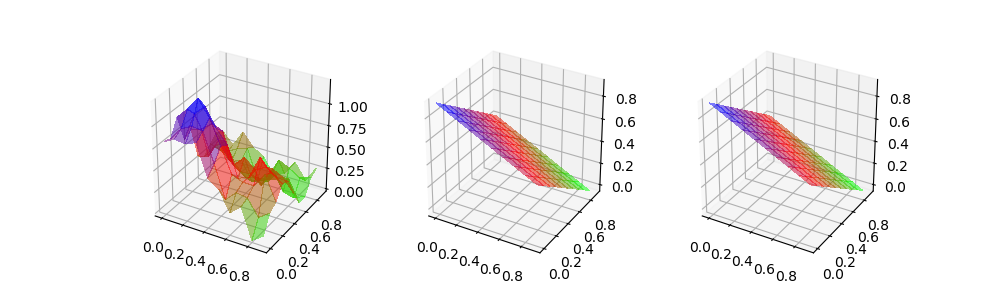
\includegraphics[width=1\linewidth]{images/surf/fake_linear_p01_n10.png}
  %\caption{}
  %\label{fig:v_x}
\end{subfigure}
\begin{subfigure}{\textwidth}
  \centering
  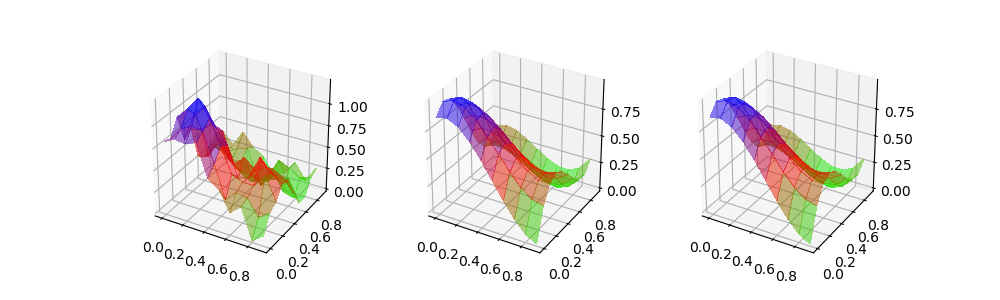
\includegraphics[width=1\linewidth]{images/surf/fake_linear_p03_n10.png}
  %\caption{}
  %\label{fig:vb_x}
\end{subfigure}
\begin{subfigure}{\textwidth}
  \centering
  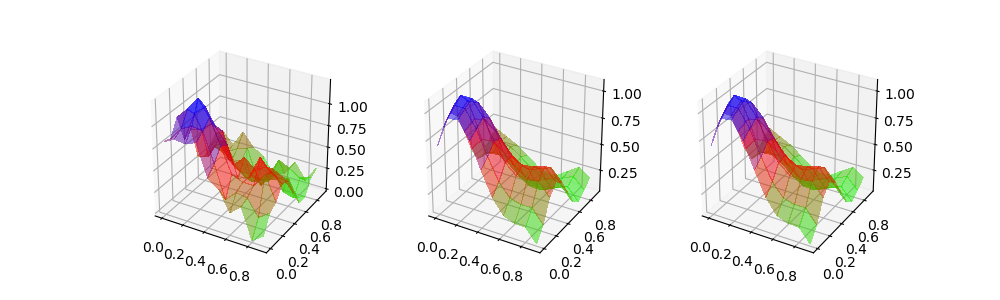
\includegraphics[width=1\linewidth]{images/surf/fake_linear_p05_n10.png}
  %\caption{}
  %\label{fig:v_x}
\end{subfigure}
\begin{subfigure}{\textwidth}
  \centering
  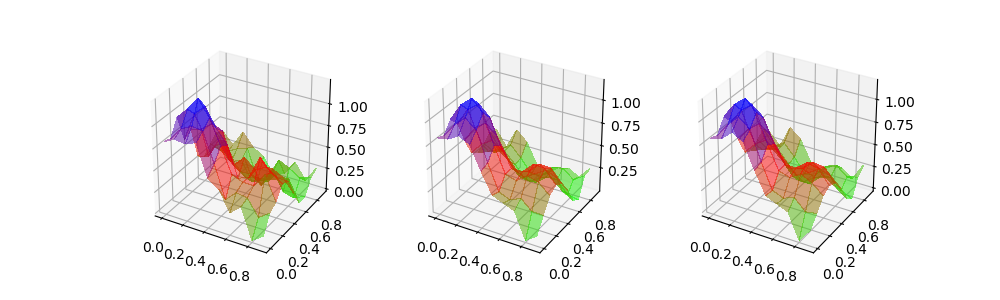
\includegraphics[width=1\linewidth]{images/surf/fake_linear_p08_n10.png}
  %\caption{}
  %\label{fig:v_x}
\end{subfigure}
\caption{The 3D visualisation of the noisy data set (left column) and the predicted surface via Lasso regression (right column) for polynomials 1, 3, 5 and 8 (from top to bottom). Grid is $10\times10$ points.}
\label{fig:linear-surf1}
\end{figure}

\begin{figure}[!ht]
\begin{subfigure}{\textwidth}
  \centering
  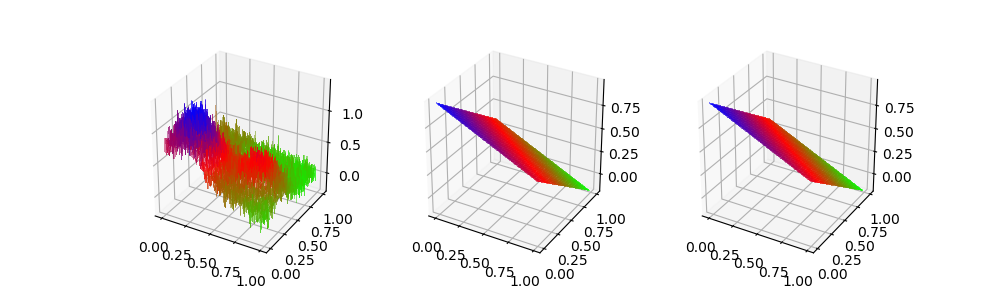
\includegraphics[width=1\linewidth]{images/surf/fake_linear_p01_n100.png}
  %\caption{}
  %\label{fig:v_x}
\end{subfigure}
\begin{subfigure}{\textwidth}
  \centering
  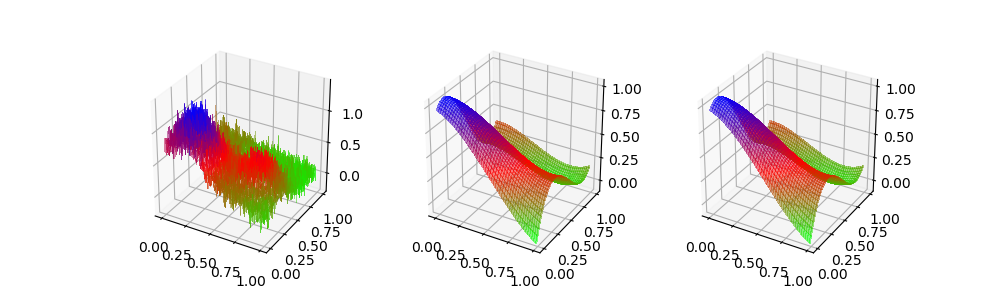
\includegraphics[width=1\linewidth]{images/surf/fake_linear_p03_n100.png}
  %\caption{}
  %\label{fig:vb_x}
\end{subfigure}
\begin{subfigure}{\textwidth}
  \centering
  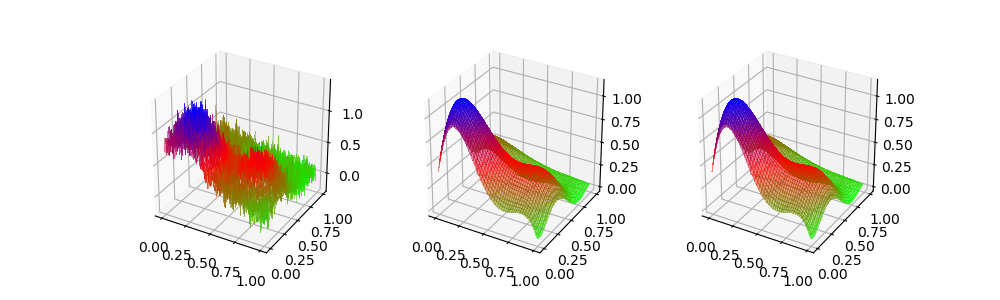
\includegraphics[width=1\linewidth]{images/surf/fake_linear_p05_n100.png}
  %\caption{}
  %\label{fig:v_x}
\end{subfigure}
\begin{subfigure}{\textwidth}
  \centering
  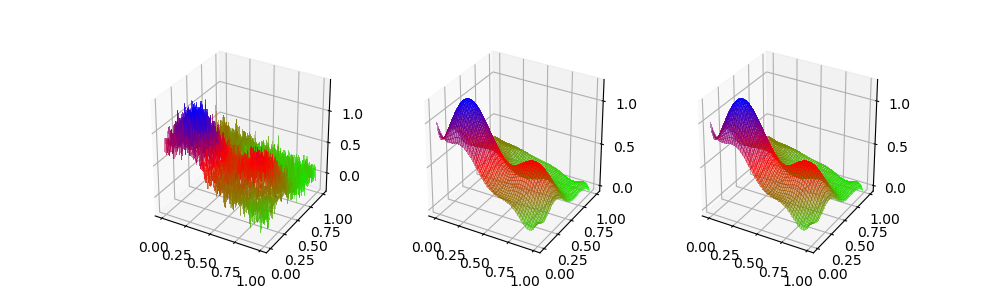
\includegraphics[width=1\linewidth]{images/surf/fake_linear_p08_n100.png}
  %\caption{}
  %\label{fig:v_x}
\end{subfigure}
\caption{The 3D visualisation of the noisy data set (left column) and the predicted surface via Lasso regression (right column) for polynomials 1, 3, 5 and 8 (from top to bottom). Grid is $100\times100$ points.}
\label{fig:linear-surf2}
\end{figure}
 
  \begin{figure}[!ht]
\begin{subfigure}{\textwidth}
  \centering
  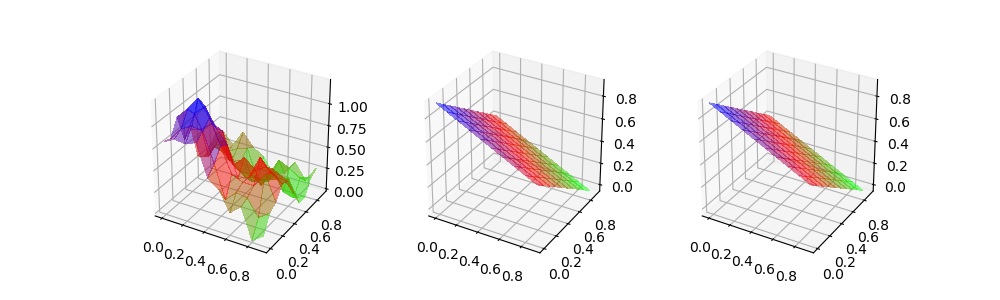
\includegraphics[width=1\linewidth]{images/surf/fake_ridge_p01_n10.png}
  %\caption{}
  %\label{fig:v_x}
\end{subfigure}
\begin{subfigure}{\textwidth}
  \centering
  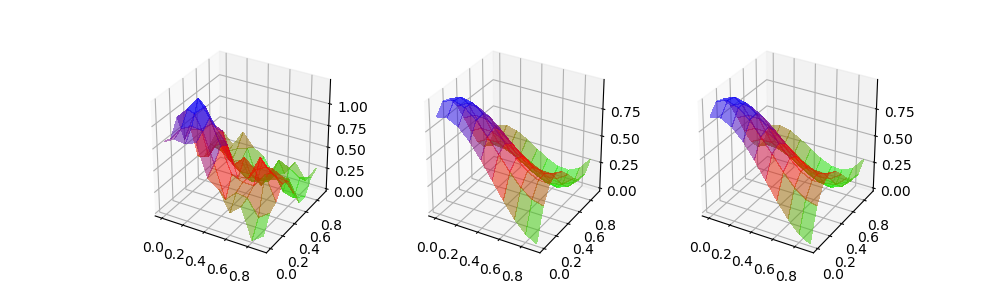
\includegraphics[width=1\linewidth]{images/surf/fake_ridge_p03_n10.png}
  %\caption{}
  %\label{fig:vb_x}
\end{subfigure}
\begin{subfigure}{\textwidth}
  \centering
  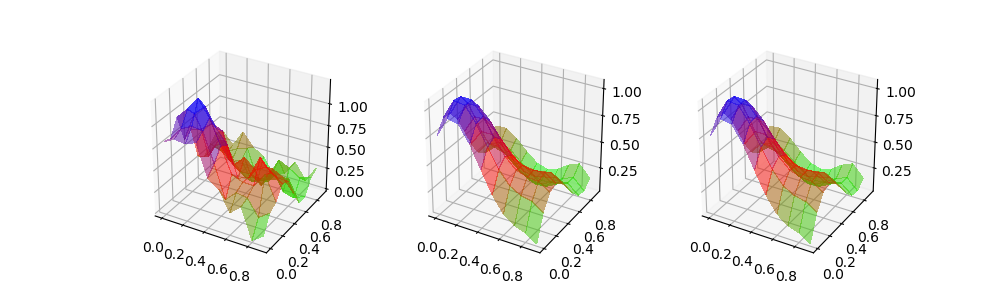
\includegraphics[width=1\linewidth]{images/surf/fake_ridge_p05_n10.png}
  %\caption{}
  %\label{fig:v_x}
\end{subfigure}
\begin{subfigure}{\textwidth}
  \centering
  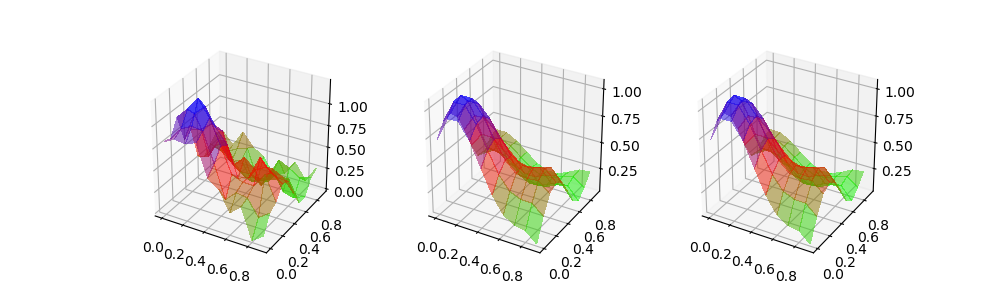
\includegraphics[width=1\linewidth]{images/surf/fake_ridge_p08_n10.png}
  %\caption{}
  %\label{fig:v_x}
\end{subfigure}
\caption{The 3D visualisation of the noisy data set (left column) and the predicted surface via Ridge regression (right column) for polynomials 1, 3, 5 and 8 (from top to bottom). Grid is $10\times10$ points and $\lambda = 0.0001$.}
\label{fig:ridge-surf1}
\end{figure}

 \begin{figure}[!ht]
\begin{subfigure}{\textwidth}
  \centering
  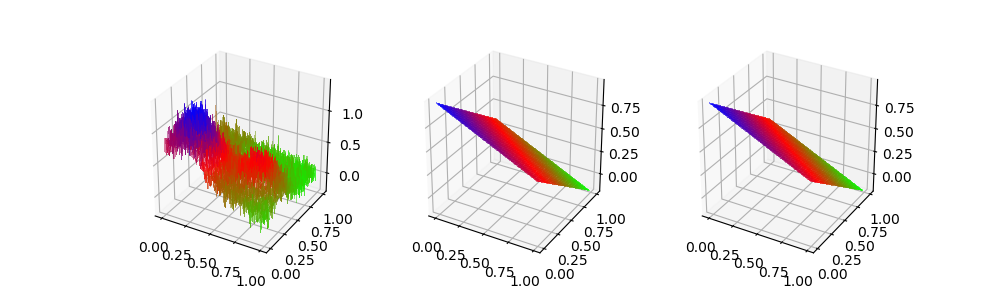
\includegraphics[width=1\linewidth]{images/surf/fake_ridge_p01_n100.png}
  %\caption{}
  %\label{fig:v_x}
\end{subfigure}
\begin{subfigure}{\textwidth}
  \centering
  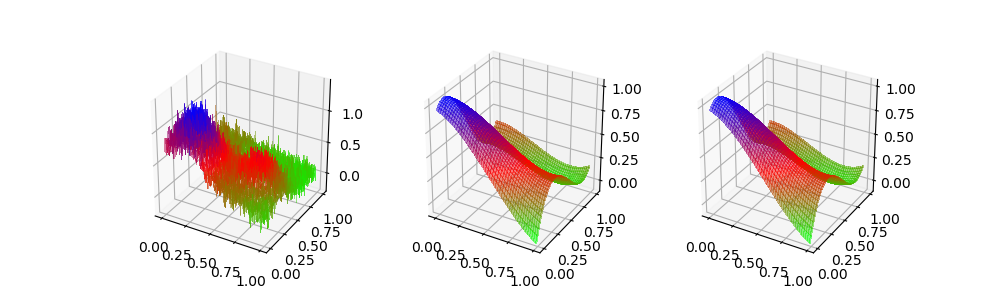
\includegraphics[width=1\linewidth]{images/surf/fake_ridge_p03_n100.png}
  %\caption{}
  %\label{fig:vb_x}
\end{subfigure}
\begin{subfigure}{\textwidth}
  \centering
  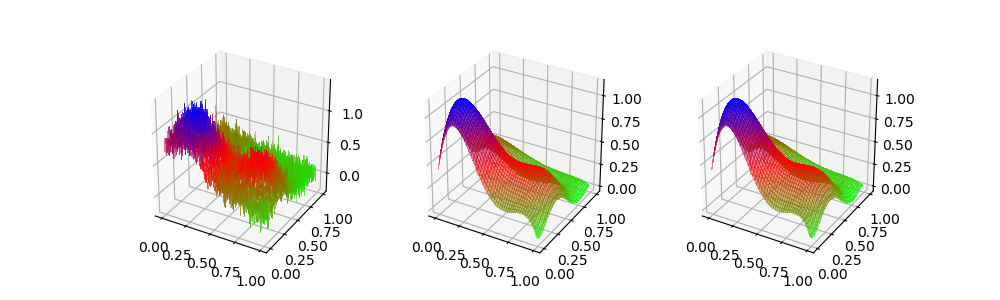
\includegraphics[width=1\linewidth]{images/surf/fake_ridge_p05_n100.png}
  %\caption{}
  %\label{fig:v_x}
\end{subfigure}
\begin{subfigure}{\textwidth}
  \centering
  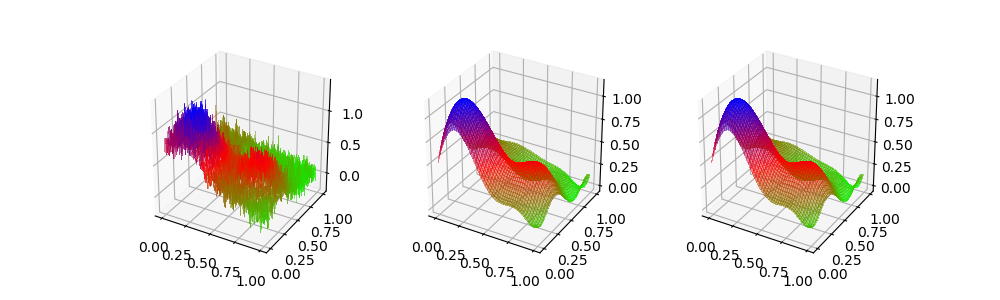
\includegraphics[width=1\linewidth]{images/surf/fake_ridge_p08_n100.png}
  %\caption{}
  %\label{fig:v_x}
\end{subfigure}
\caption{The 3D visualisation of the noisy data set (left column) and the predicted surface via Ridge regression (right column) for polynomials 1, 3, 5 and 8 (from top to bottom). Grid is $100\times100$ points and $\lambda = 0.0001$.}
\label{fig:ridge-surf2}
\end{figure}
 
\begin{figure}[!ht]
\begin{subfigure}{\textwidth}
  \centering
  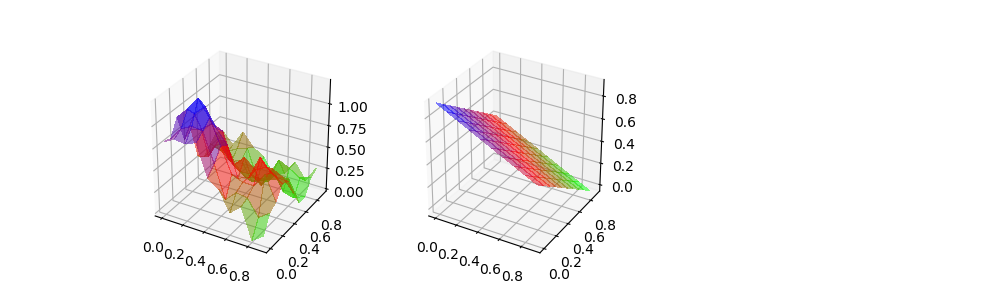
\includegraphics[width=1\linewidth]{images/surf/fake_lasso_p01_n10.png}
  %\caption{}
  %\label{fig:v_x}
\end{subfigure}
\begin{subfigure}{\textwidth}
  \centering
  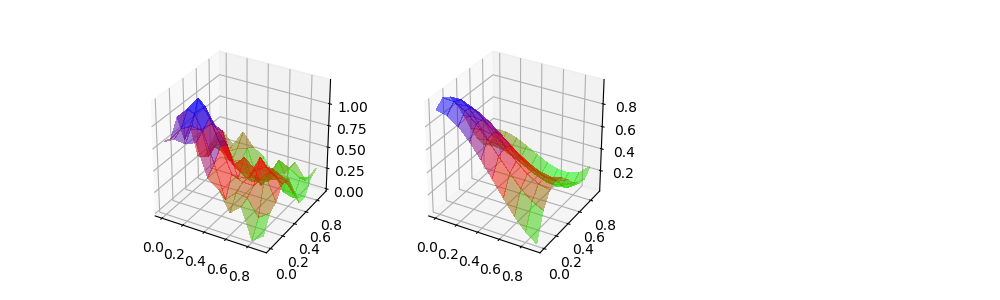
\includegraphics[width=1\linewidth]{images/surf/fake_lasso_p03_n10.png}
  %\caption{}
  %\label{fig:vb_x}
\end{subfigure}
\begin{subfigure}{\textwidth}
  \centering
  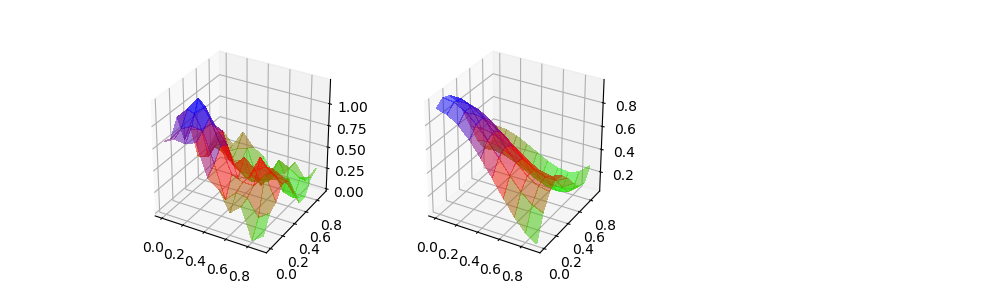
\includegraphics[width=1\linewidth]{images/surf/fake_lasso_p05_n10.png}
  %\caption{}
  %\label{fig:v_x}
\end{subfigure}
\begin{subfigure}{\textwidth}
  \centering
  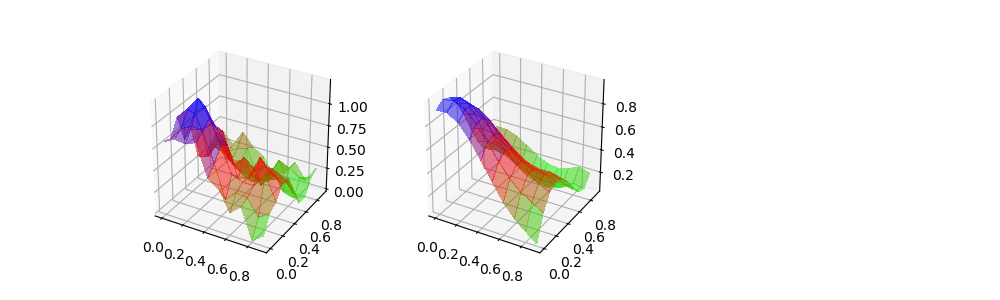
\includegraphics[width=1\linewidth]{images/surf/fake_lasso_p08_n10.png}
  %\caption{}
  %\label{fig:v_x}
\end{subfigure}
\caption{The 3D visualisation of the noisy data set (left column) and the predicted surface via Lasso regression (right column) for polynomials 1, 3, 5 and 8 (from top to bottom). Grid is $10\times10$ points and $\lambda = 0.0001$.}
\label{fig:lasso-surf1}
\end{figure}

\begin{figure}[!ht]
\begin{subfigure}{\textwidth}
  \centering
  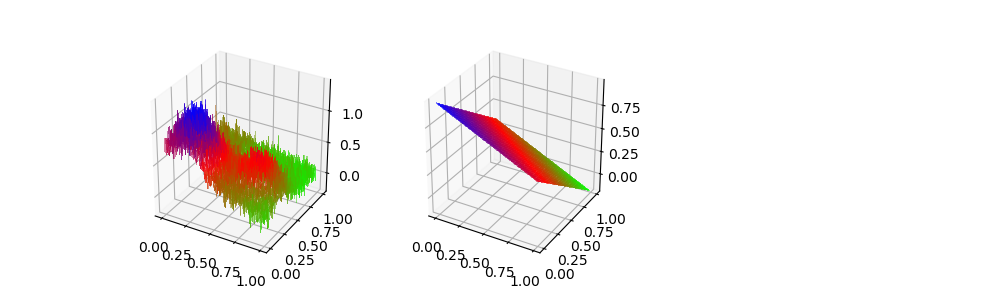
\includegraphics[width=1\linewidth]{images/surf/fake_lasso_p01_n100.png}
  %\caption{}
  %\label{fig:v_x}
\end{subfigure}
\begin{subfigure}{\textwidth}
  \centering
  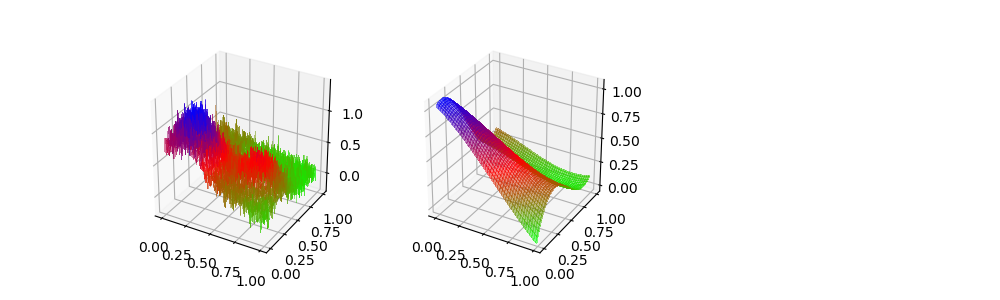
\includegraphics[width=1\linewidth]{images/surf/fake_lasso_p03_n100.png}
  %\caption{}
  %\label{fig:vb_x}
\end{subfigure}
\begin{subfigure}{\textwidth}
  \centering
  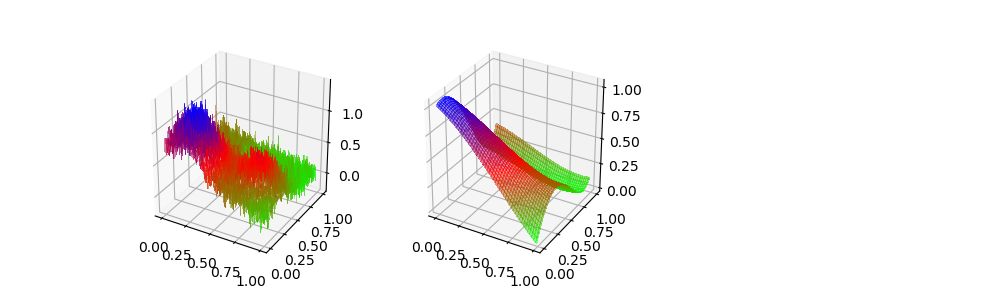
\includegraphics[width=1\linewidth]{images/surf/fake_lasso_p05_n100.png}
  %\caption{}
  %\label{fig:v_x}
\end{subfigure}
\begin{subfigure}{\textwidth}
  \centering
  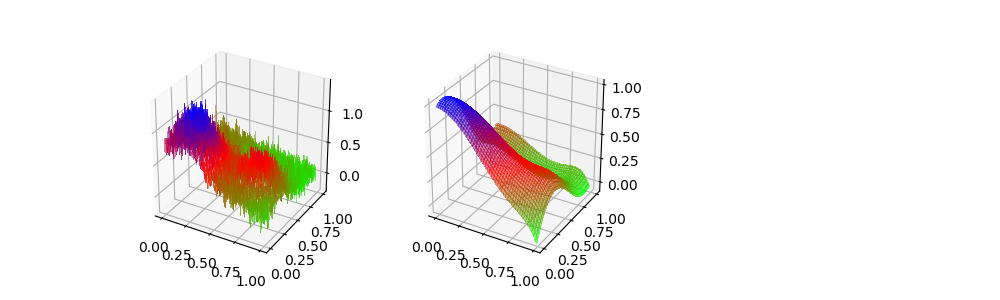
\includegraphics[width=1\linewidth]{images/surf/fake_lasso_p08_n100.png}
  %\caption{}
  %\label{fig:v_x}
\end{subfigure}
\caption{The 3D visualisation of the noisy data set (left column) and the predicted surface via Lasso regression (right column) for polynomials 1, 3, 5 and 8 (from top to bottom). Grid is $100\times100$ points and $\lambda = 0.0001$.}
\label{fig:lasso-surf2}
\end{figure}

%%%%%%%%%%%%%%%%%%%%%%%%%%%%%%%%%%%%%%%%%%%%%%%%%%%%%%%%%%%%%%%%%%%%%%%%%%%%%%%%%%%%%
% betas
%%%%%%%%%%%%%%%%%%%%%%%%%%%%%%%%%%%%%%%%%%%%%%%%%%%%%%%%%%%%%%%%%%%%%%%%%%%%%%%%%%%%%

\begin{figure}[!ht]
\begin{subfigure}{\textwidth}
  \centering
  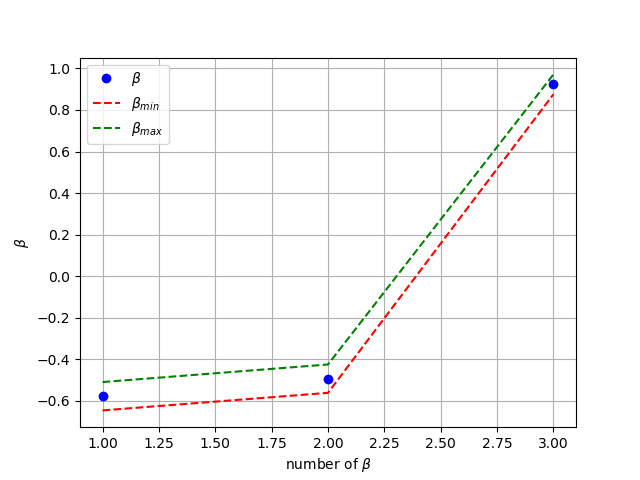
\includegraphics[width=0.5\linewidth]{images/betas/fake_linear_beta_p01_n10.png}
  %\caption{}
  %\label{fig:v_x}
\end{subfigure}
\begin{subfigure}{\textwidth}
  \centering
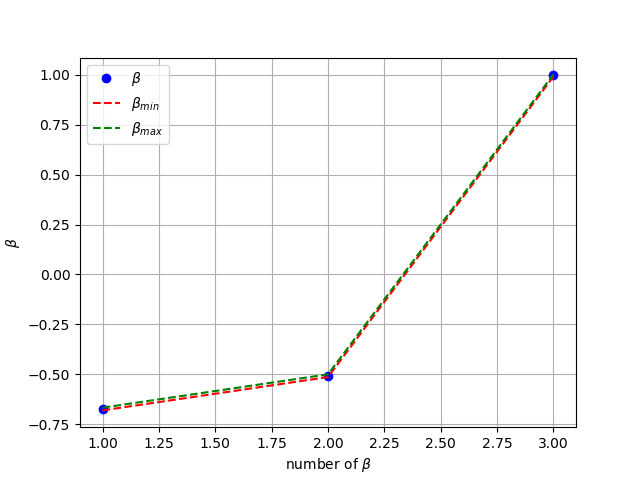
\includegraphics[width=0.5\linewidth]{images/betas/fake_linear_beta_p01_n100.png}
  %\caption{}
  %\label{fig:vb_x}
\end{subfigure}
\begin{subfigure}{\textwidth}
  \centering
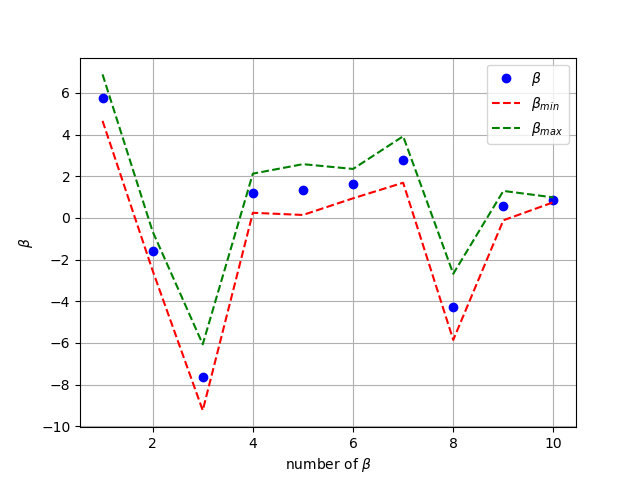
\includegraphics[width=0.5\linewidth]{images/betas/fake_linear_beta_p03_n10.png}
  %\caption{}
  %\label{fig:v_x}
\end{subfigure}
\begin{subfigure}{\textwidth}
  \centering
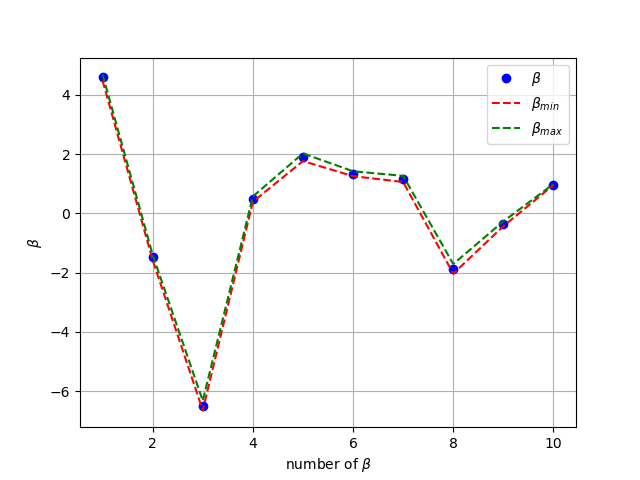
\includegraphics[width=0.5\linewidth]{images/betas/fake_linear_beta_p03_n100.png}
  %\caption{}
  %\label{fig:v_x}
\end{subfigure}
\begin{subfigure}{\textwidth}
  \centering
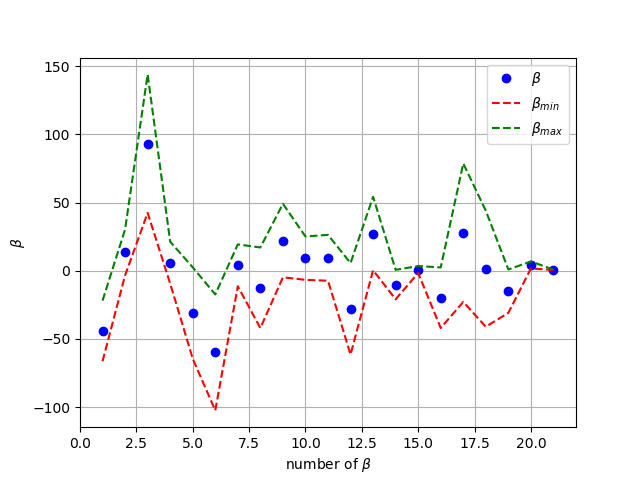
\includegraphics[width=0.5\linewidth]{images/betas/fake_linear_beta_p05_n10.png}
  %\caption{}
  %\label{fig:v_x}
\end{subfigure}
\begin{subfigure}{\textwidth}
  \centering
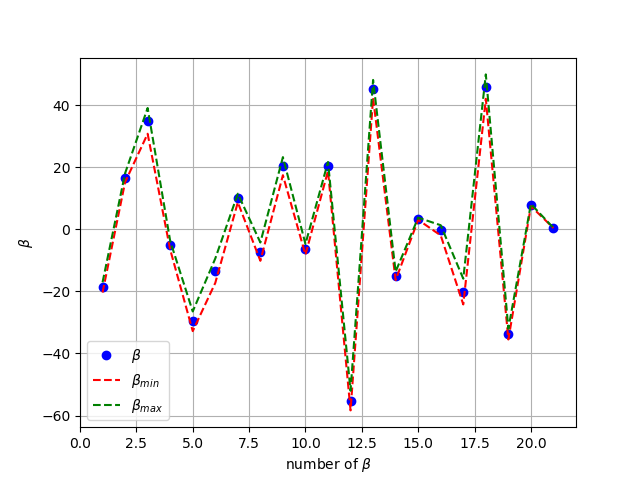
\includegraphics[width=0.5\linewidth]{images/betas/fake_linear_beta_p05_n100.png}
  %\caption{}
  %\label{fig:v_x}
\end{subfigure}
\begin{subfigure}{\textwidth}
  \centering
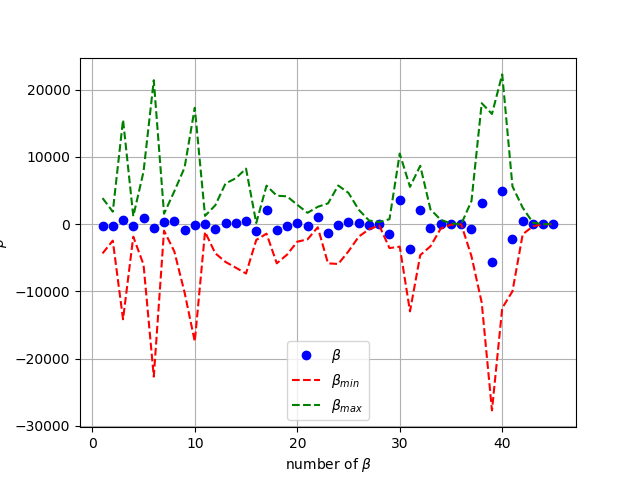
\includegraphics[width=0.5\linewidth]{images/betas/fake_linear_beta_p08_n10.png}
  %\caption{}
  %\label{fig:v_x}
\end{subfigure}
\begin{subfigure}{\textwidth}
  \centering
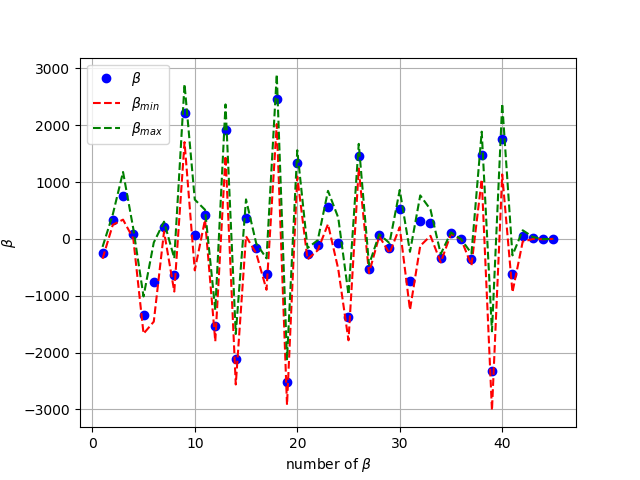
\includegraphics[width=0.5\linewidth]{images/betas/fake_linear_beta_p08_n100.png}
  %\caption{}
  %\label{fig:v_x}
\end{subfigure}
\caption{Manually calculated parameters $\beta$ of Linear Regression model for polynomials 1, 3, 5 and 8 (from top to bottom) on the grids $10\times10$ (left column) and $100\times100$ (right column) points.}
\label{fig:linear-beta}
\end{figure}

\begin{figure}[!ht]
\begin{subfigure}{\textwidth}
  \centering
  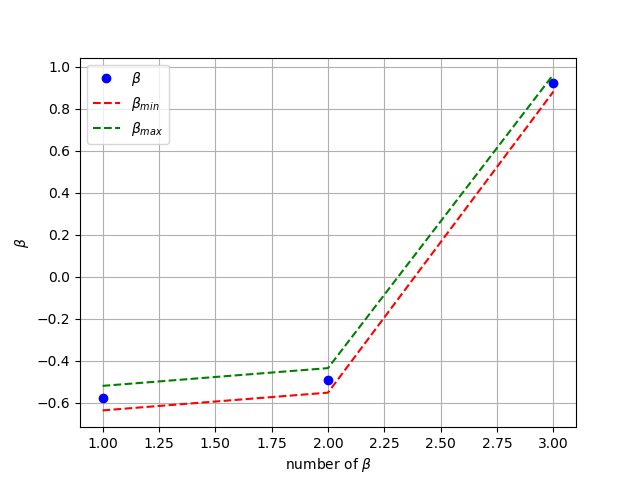
\includegraphics[width=0.5\linewidth]{images/betas/fake_ridge_beta_p01_n10.png}
  %\caption{}
  %\label{fig:v_x}
\end{subfigure}
\begin{subfigure}{\textwidth}
  \centering
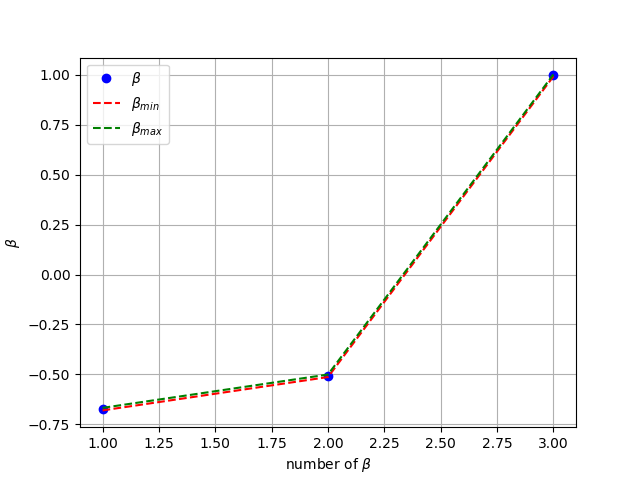
\includegraphics[width=0.5\linewidth]{images/betas/fake_ridge_beta_p01_n100.png}
  %\caption{}
  %\label{fig:vb_x}
\end{subfigure}
\begin{subfigure}{\textwidth}
  \centering
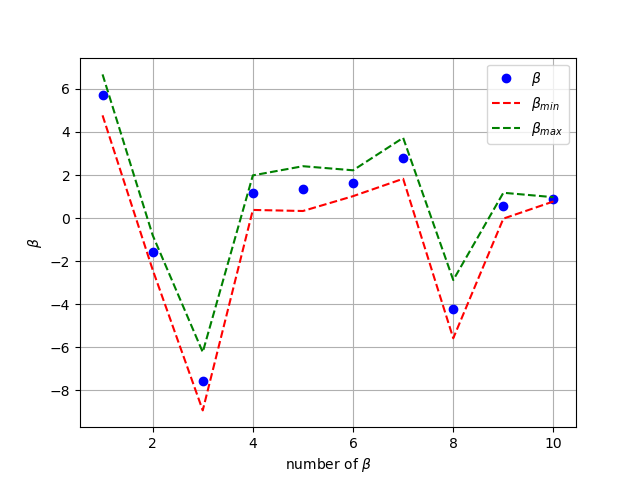
\includegraphics[width=0.5\linewidth]{images/betas/fake_ridge_beta_p03_n10.png}
  %\caption{}
  %\label{fig:v_x}
\end{subfigure}
\begin{subfigure}{\textwidth}
  \centering
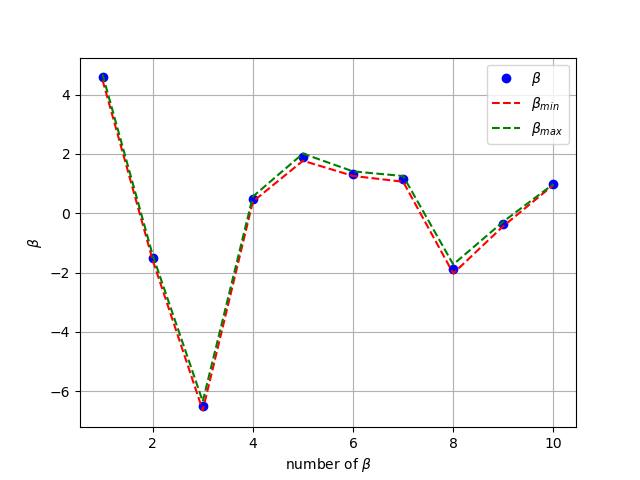
\includegraphics[width=0.5\linewidth]{images/betas/fake_ridge_beta_p03_n100.png}
  %\caption{}
  %\label{fig:v_x}
\end{subfigure}
\begin{subfigure}{\textwidth}
  \centering
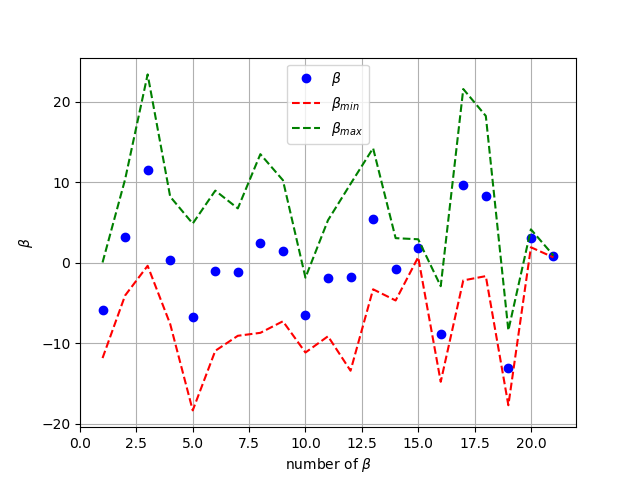
\includegraphics[width=0.5\linewidth]{images/betas/fake_ridge_beta_p05_n10.png}
  %\caption{}
  %\label{fig:v_x}
\end{subfigure}
\begin{subfigure}{\textwidth}
  \centering
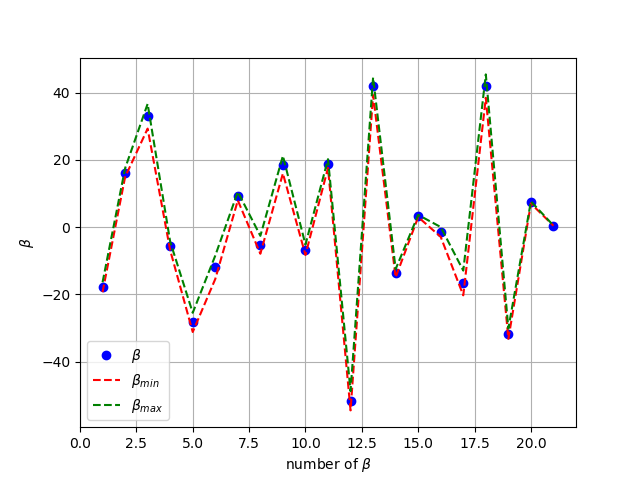
\includegraphics[width=0.5\linewidth]{images/betas/fake_ridge_beta_p05_n100.png}
  %\caption{}
  %\label{fig:v_x}
\end{subfigure}
\begin{subfigure}{\textwidth}
  \centering
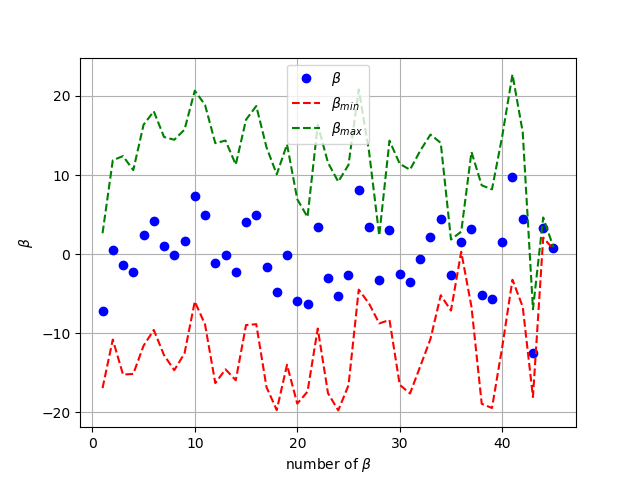
\includegraphics[width=0.5\linewidth]{images/betas/fake_ridge_beta_p08_n10.png}
  %\caption{}
  %\label{fig:v_x}
\end{subfigure}
\begin{subfigure}{\textwidth}
  \centering
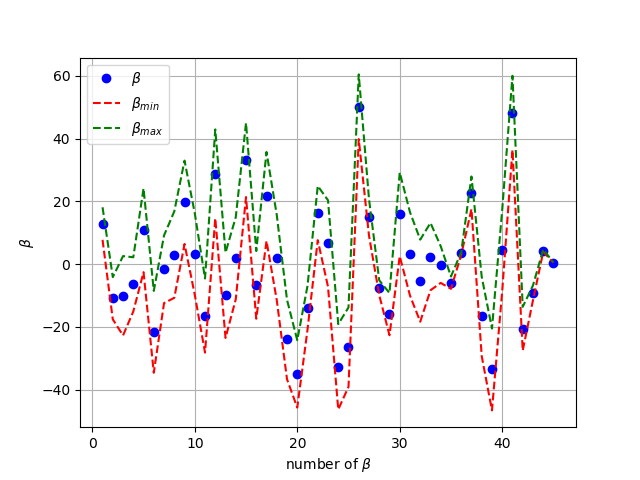
\includegraphics[width=0.5\linewidth]{images/betas/fake_ridge_beta_p08_n100.png}
  %\caption{}
  %\label{fig:v_x}
\end{subfigure}
\caption{Manually calculated parameters $\beta$ of Ridge Regression model for polynomials 1, 3, 5 and 8 (from top to bottom) on the grids $10\times10$ (left column) and $100\times100$ (right column) points. $\lambda = 0.0001$.}
\label{fig:ridge-beta}
\end{figure}

Figures \ref{fig:linear-beta} and \ref{fig:ridge-beta} clearly state that the more points we have in the data set, the less uncertain we be about out model parameters.


Unfortunately, all these values cannot say for sure whether we will fit future data sets correctly (our main goal is to create such model) or not. That is why, as was discussed in the previous sections, we need to consider a resampling techniques. 

 \subsubsection{Resampling techniques: Bias-variance tradeoff}
 
 In section \ref{} I have described implementation of kFold Cross Validation Algorithm; thus, below I present the main results for the specified runs.
 
 Figure \rf{} shows that when the amount of points increases the closer test slope appears to be to the white noise threshold (in our case supposed to be at $\sigma^2=0.01$), and less diverge it from the train values. On the contrary, the less amount of points we have the more evident is the \textit{bias-variance trade-off}: the area to the left is the \textit{High Bias} (\textit{Low Variance}) zone, whereas with the increase of model complexity the curves are diverging, while entering \textit{Low Bias} (\textit{High Variance}) zone.
 
 %%%%%%%%%%%%%%%%%%%%%%%%%%%%%%%%%%%%%%%%%%%%%%%%%%%%%%%%%%%%%%%%%%%%%%%%%%%%%%%%%%%%%
 % MSE
 %%%%%%%%%%%%%%%%%%%%%%%%%%%%%%%%%%%%%%%%%%%%%%%%%%%%%%%%%%%%%%%%%%%%%%%%%%%%%%%%%%%%%
\begin{figure}[!ht]
\begin{subfigure}{\textwidth}
  \centering
  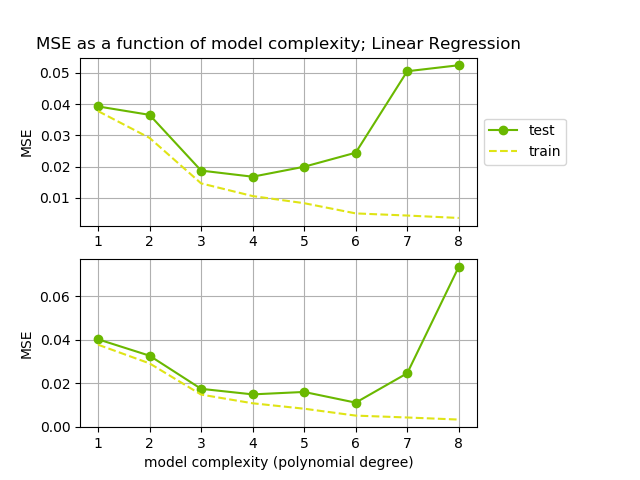
\includegraphics[width=0.55\linewidth]{images/mse/fake_linear_mse_p08_n10.png}
  %\caption{$10\times10$}
  %\label{fig:v_x}
\end{subfigure}
\begin{subfigure}{\textwidth}
  \centering
  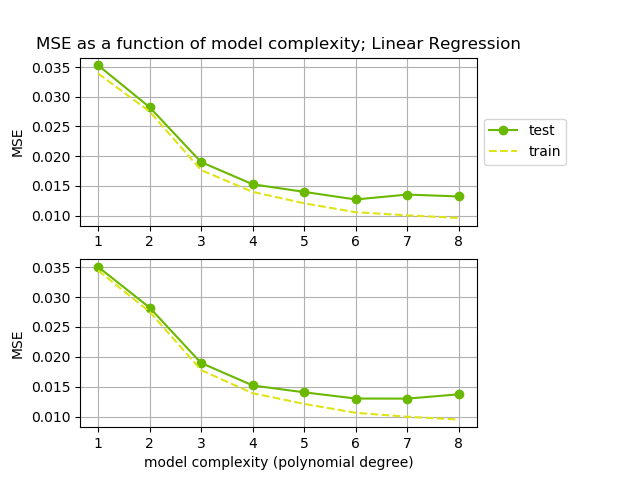
\includegraphics[width=0.55\linewidth]{images/mse/fake_linear_mse_p08_n21.png}
  %\caption{$21\times21$}
  %\label{fig:vb_x}
\end{subfigure}
\begin{subfigure}{\textwidth}
  \centering
  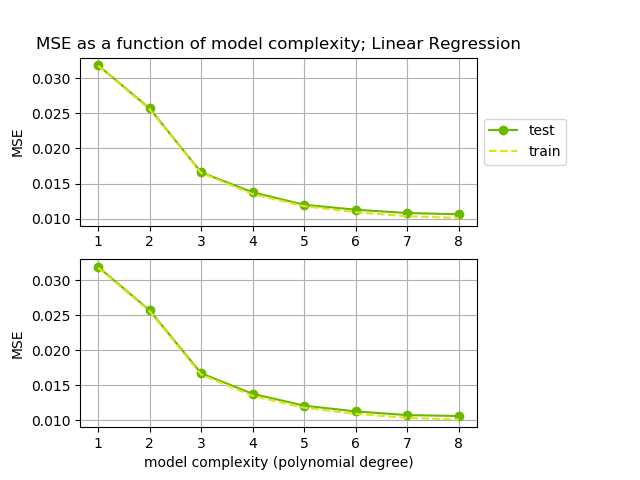
\includegraphics[width=0.55\linewidth]{images/mse/fake_linear_mse_p08_n50.png}
  %\caption{$50\times50$}
  %\label{fig:vb_x}
\end{subfigure}
\begin{subfigure}{\textwidth}
  \centering
  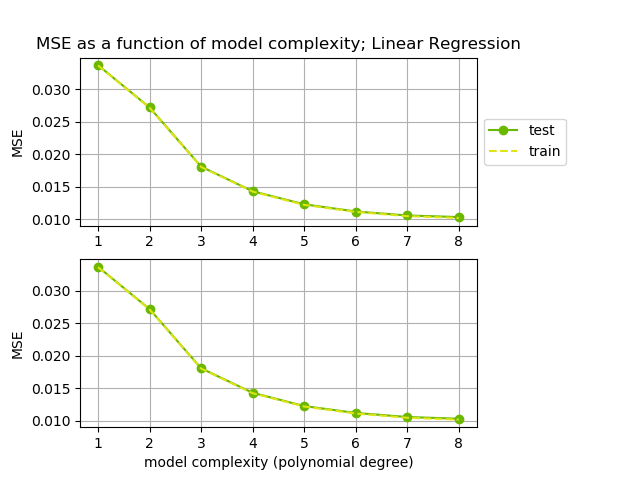
\includegraphics[width=0.55\linewidth]{images/mse/fake_linear_mse_p08_n100.png}
  %\caption{$100\times100$}
  %\label{fig:vb_x}
\end{subfigure}
\caption{MSE plot of train and test data sets as a function of model complexity (polynomial degree) calculated via Linear Regression for several different grids: $10\times10$ (top left), $21\times21$ (top right), $50\times50$ (bottom left), $100\times100$ (bottom right).}
\label{fig:linear-mse}
\end{figure}

\begin{figure}[!ht]
\begin{subfigure}{\textwidth}
  \centering
  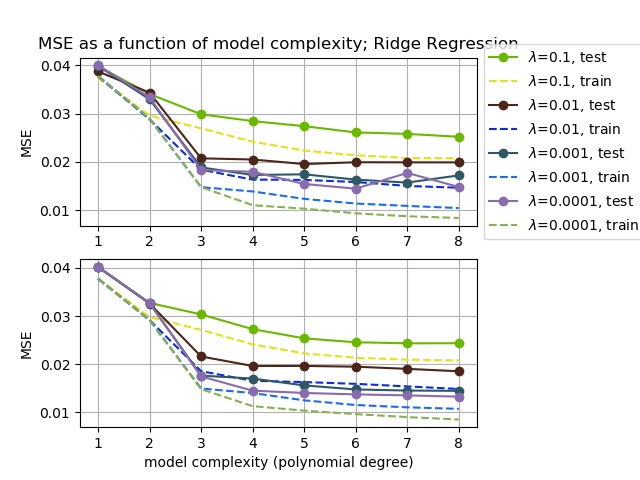
\includegraphics[width=0.55\linewidth]{images/mse/fake_ridge_mse_p08_n10.png}
  %\caption{$10\times10$}
  %\label{fig:v_x}
\end{subfigure}
\begin{subfigure}{\textwidth}
  \centering
  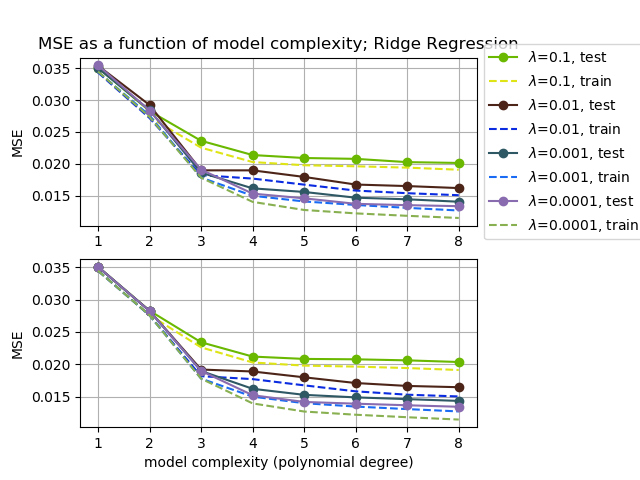
\includegraphics[width=0.55\linewidth]{images/mse/fake_ridge_mse_p08_n21.png}
  %\caption{$21\times21$}
  %\label{fig:vb_x}
\end{subfigure}
\begin{subfigure}{\textwidth}
  \centering
  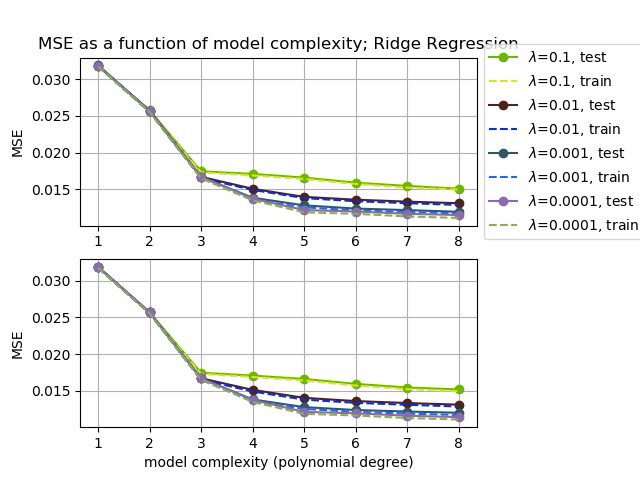
\includegraphics[width=0.55\linewidth]{images/mse/fake_ridge_mse_p08_n50.png}
  %\caption{$50\times50$}
  %\label{fig:vb_x}
\end{subfigure}
\begin{subfigure}{\textwidth}
  \centering
  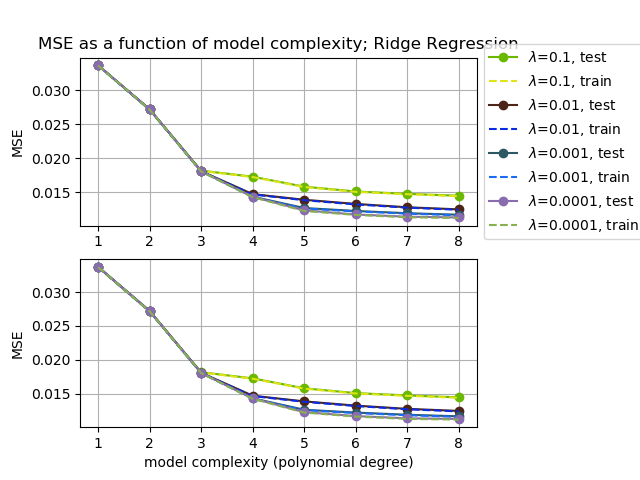
\includegraphics[width=0.55\linewidth]{images/mse/fake_ridge_mse_p08_n100.png}
  %\caption{$100\times100$}
  %\label{fig:vb_x}
\end{subfigure}
\caption{MSE plot of train and test data sets as a function of model complexity (polynomial degree) calculated via Ridge Regression for several different grids: $10\times10$ (top left), $21\times21$ (top right), $50\times50$ (bottom left), $100\times100$ (bottom right). $\lambda_i = 0.1$, $0.01$ and $0.0001$.}
\label{fig:ridge-mse}
\end{figure}

\begin{figure}[!ht]
\begin{subfigure}{\textwidth}
  \centering
  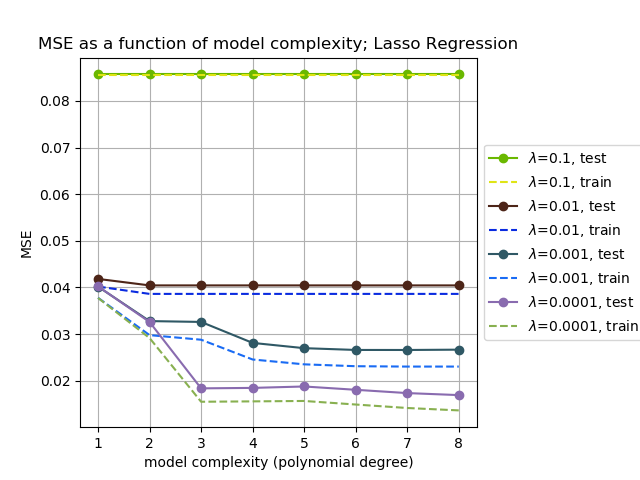
\includegraphics[width=0.55\linewidth]{images/mse/fake_lasso_mse_p08_n10.png}
  %\caption{$10\times10$}
  %\label{fig:v_x}
\end{subfigure}
\begin{subfigure}{\textwidth}
  \centering
  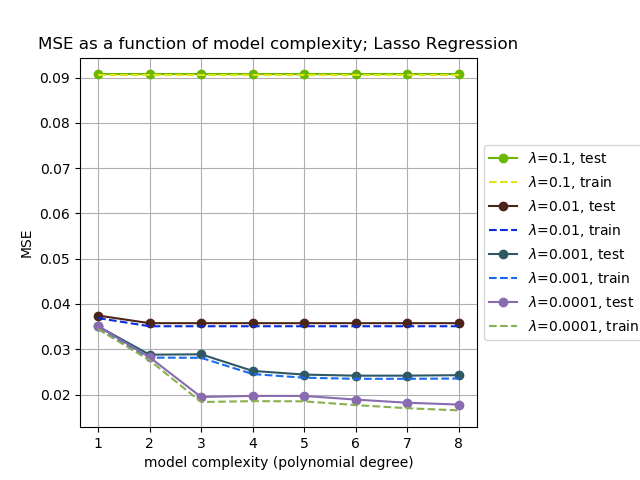
\includegraphics[width=0.55\linewidth]{images/mse/fake_lasso_mse_p08_n21.png}
  %\caption{$21\times21$}
  %\label{fig:vb_x}
\end{subfigure}
\begin{subfigure}{\textwidth}
  \centering
  \includegraphics[width=0.55\linewidth]{images/mse/fake_lasso_mse_p08_n50.png}
  %\caption{$50\times50$}
  %\label{fig:vb_x}
\end{subfigure}
\begin{subfigure}{\textwidth}
  \centering
  \includegraphics[width=0.55\linewidth]{images/mse/fake_lasso_mse_p08_n100.png}
  %\caption{$100\times100$}
  %\label{fig:vb_x}
\end{subfigure}
\caption{MSE plot of train and test data sets as a function of model complexity (polynomial degree) calculated via Lasso Regression for several different grids: $10\times10$ (top left), $21\times21$ (top right), $50\times50$ (bottom left), $100\times100$ (bottom right). $\lambda_i = 0.1$, $0.01$ and $0.0001$.}
\label{fig:lasso-mse}
\end{figure}

As we can see from figure \rf{}, the closer hyper parameter to zero, the closer the values of Ridge regression correlate with the values from Linear regression. And vice versa, the closer $\lambda$ to 1, the more straight our line appear to be - this is nothing surprising, as setting $\lambda=1$ equivalent to setting $\beta\rightarrow\infty$ (?) <= to zero (check lasso once again, it should be zero).

The figure \rf{} shows MSE for training and test data sets, calculated via Lasso regression and kFold cross validation, when I split data sets into 5 folds. It is evident that Lasso appears to be more dependent on hyper parameter, then Ridge regression.

From a student view about Lasso:
\textit{"The problem is that there is no problem. This is just truly what the data is like: the dataset is so large that the signal to noise ratio is very high, this means that even with high polynomial orders you never overfit (because you have so much training and test data that they become very similar).}

\texdtit{When we use a lot smaller amount of data points, for example 500, then we see the expected result where the test error goes up after a number of rounds.}

\textit{It makes sense that when you turn off shuffle the training and test error increases: without shuffle, the training data is one part of the image, and the test data a different part of the image. Obviously you can not "learn" something that you have not seen."}




 \subsection{Real Data}
 
 Below I present main results for the real data set. I run script up til 5th polynomial degree with several different hyper parameters.
 
 \begin{figure}[!ht]
\begin{subfigure}{\textwidth}
  \centering
  \includegraphics[width=1.2\linewidth]{images/surf/fake_lasso_p01_n50.png}
  %\caption{}
  %\label{fig:v_x}
\end{subfigure}
\begin{subfigure}{\textwidth}
  \centering
  \includegraphics[width=1.2\linewidth]{images/surf/fake_lasso_p03_n50.png}
  %\caption{}
  %\label{fig:vb_x}
\end{subfigure}
\begin{subfigure}{\textwidth}
  \centering
  \includegraphics[width=1.2\linewidth]{images/surf/fake_lasso_p05_n50.png}
  %\caption{}
  %\label{fig:v_x}
\end{subfigure}
\caption{The 3D visualisation of the noisy data set (left column) and the predicted surface via Lasso regression (right column) for polynomials 1, 3, 5 and 8 (from top to bottom). Grid is $50\times50$ points and $\lambda = 0.0001$.}
\label{fig:lasso-surf}
\end{figure}
 
 \subsection{Future Improvements}
 
 This question is more of general nature, where I mostly summarize the things which would be good to implement, but due to lack of time was not implemented:
 
 - Tuning of the Ridge and lasso, e.g. GridSearchCV
 - Reduce the size of the data set, without losing the information. Huffman coding as a solution?
 - Add features which will support any type of input function (say with n independent variables - it can be an input one) <= would be fun.
 - The Multiprocessing was implemented, but it is not perfect <= think of a better way to do it;
 
 As one of the future improvements, It woulde be better to implement the tuning of the Ridge and Lasso models. To be more precise, generate, say, hundred $\lambda$ values and find the corresponding MSEs for each of them. after that, find the minimal one out of 100 generated - this value will be give us the best $\lambda$ value for Ridge and Lasso Regressions. I wanted to implement this feature already, but due to the high value of real data sets, it will take a lot of time to converge even for one polynomial. 
 
 One of the students suggest reduce the size of the data set without losing information. Perhaps, it is good approach in general, say use Huffman coding or something similar ?

